\chapter{User Manual}
\label{ch:usermanual}

	\todo{We probably need health disclaimers somewhere in our doc?}

	\section{Welcome}
	\label{sec:welcome}

		\begin{wrapfigure}{R}{0.25\textwidth}
			\vspace{-5em}
			\centering
			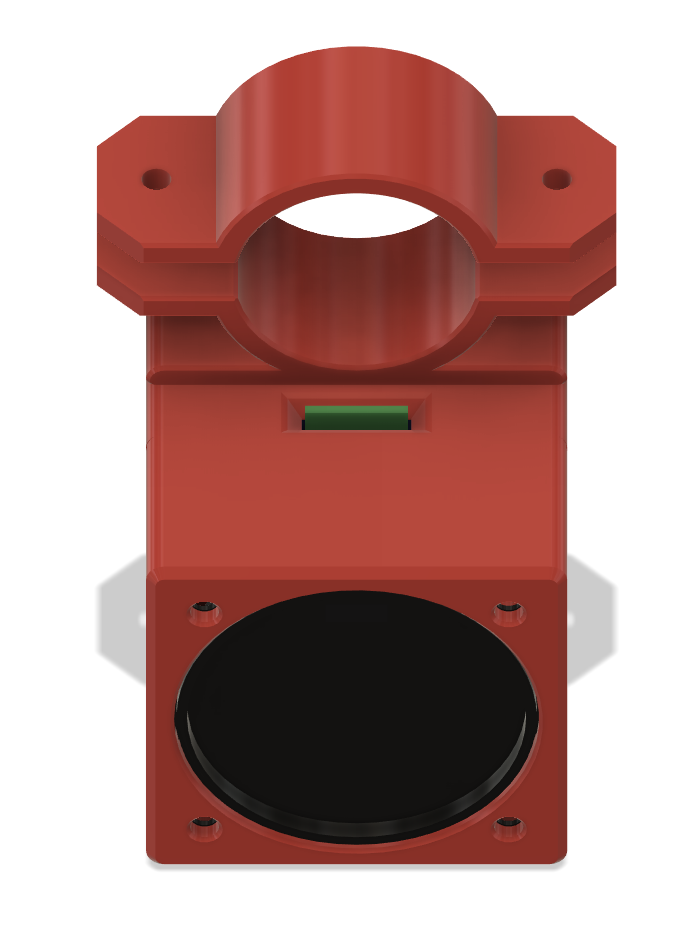
\includegraphics[width=0.25\textwidth]{graphics/final-cad.png}
		\end{wrapfigure}

		The Walking Aid Usage Prompt System is a medical aid consisting of a pair of hardware devices that allows patients suffering with dementia to be automatically reminded to use their walking aid when they begin walking without it. With stastically high rates of falling in dementia patients, the Walking Aid Usage Prompt System attempts to reduce these numbers. It aims to do this by detecting when patients are walking without their walking aid and plays them an audible reminder from a relatives voice, to take their walking aid with them.

		\paragraph{Automatic Movement Detection}\mbox{}

		With the use of an accelerometer in each device, our systems can automatically detect when your patient is moving, and if they are moving without their walking aid.

		\paragraph{Remind the patient with the sound of a familiar voice}\mbox{}

		Utilising the SD card reader on the walking aid device, you can upload an MP3 file to be played to the patient when they begin walking without their walking aid. The connected speaker will give you the peace of mind that the patient will hear the reminder whenever it needs to be played. According to our research, and insight from the client, this will increase the chances of the patient reacting appropriately, and will ease them into being accustomed to the device.

		\begin{wrapfigure}[6]{L}{0.25\textwidth}
			\vspace{-1em}
			\centering
			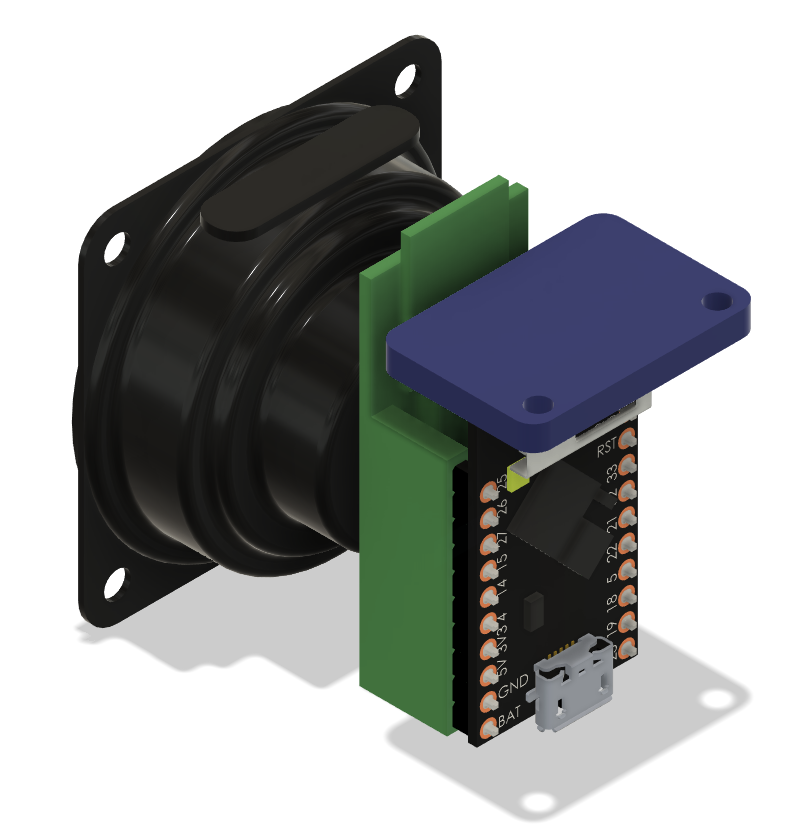
\includegraphics[width=0.25\textwidth]{graphics/hardware.png}
		\end{wrapfigure}

		\paragraph{Use vibration feedback as a reminder for patients who are hard of hearing}\mbox{}

		The inclusion of a low power, low latency communication protocol between our two devices will mean that the use of an audio reminder can be replaced, with the wearable device being asked to vibrate instead.

		\newpage

		\paragraph{Never use intrusive wearables again}\mbox{}

		Boasting a small form factor and the avoidance of distracting LEDs, our devices were developed with the comfort of the patient in mind. Utilising 18mm x 32mm TinyPICO development boards, our solution succeeds at keeping device sizes to a minimum and can be worn on either the ankle or wrist, with adaptable attachment methods that can be tailored to each patient.

		\vspace{5em}
		\paragraph{Next Steps:}\mbox{}

		\vspace{1em}
		Excited to get started?

		\textit{\hyperref[sec:quick_start_guide]{Click here for our Quick Start Guide} or head to section \ref{sec:quick_start_guide}}

		\vspace{1em}
		Want to learn more?

		\textit{\hyperref[sec:user_guide]{Click here for our more in depth User Guide} or head to section \ref{sec:user_guide}}

		\vspace{1em}
		Are you a developer?

		\textit{\hyperref[sec:developer_guide]{Click here to head to our developer guide} or head to section \ref{sec:developer_guide}}

	\newpage
	\section{Quick Start Guide}
	\label{sec:quick_start_guide}

		\subsection{Introduction}
		\label{subsec:quick_start_guide_introduction}

			The Walking Aid Usage Prompt system is a medical aid that allows patients to be automatically reminded to use their walking aid when they begin walking without it. The whole system comprises of two separate devices, one to be attached to the user's walking aid and the other to the ankle or wrist of the user. The wearable device is used to detect when the user has taken 5 steps within a 10 second period to signify that the user has began walking. Once this occurs, the wearable device communicates with the user's walking aid device to make a check to see if the walking aid is moving also. If the walking aid is moving, then great! There is no need to worry, the user is making use of their walking aid. However, should a user not be utilising their walking aid, then the walking aid can either play an audio reminder to the user, or it can communicate back to the wearable device to vibrate against the ankle or the wrist of the user. Both solutions are designed to remind the user to take their walking aid with them when walking in an attempt to reduce fall rates in dementia patients.

			The remainder of this quick start guide will explain the prerequisites to ensure that the system is fully functional, and a brief setup guide so that the user can get started.

		\subsection{Hardware Requirements}
		\label{subsec:quick_start_guide_hardware}

			\paragraph{To use the audio reminder system:}\mbox{}

			\begin{itemize}
				\item MicroSD Card >= 2MB Capacity.
				\item Windows/MacOS/Linux Computer System.
				\item A means to read/write to the SD card from the computer system. For example, a USB to MicroSD card reader.
				\item A microphone to record audio, or a pre-recorded audio file (.MP3)
			\end{itemize}

			\paragraph{To use the vibration reminder system:}\mbox{}

			No additional hardware necessary, please advance to section \ref{subsec:quick_start_setup_guide}.

		\subsection{Software Requirements}
		\label{subsec:quick_start_guide_software}

			\paragraph{To use the audio reminder system:}\mbox{}

			\begin{itemize}
				\item Voice recording software such as Windows Voice Recorder or Audacity. (An alternative could be to record your voice message on a mobile device and transfer it to the computer system).
				\item File explorer software to copy the file to the SD card.
				\item MP3 audio file should be <= 2MB in size.
			\end{itemize}

			\paragraph{To use the vibration reminder system:}\mbox{}

			No additional software necessary, please advance to section \ref{subsec:quick_start_setup_guide}.

		\subsection{Setup Guide}
		\label{subsec:quick_start_setup_guide}

			\subsubsection{To use the audio reminder system}

				\paragraph{Getting your MicroSD card ready}\mbox{}

				To utilise the audio reminder system, you will need a MicroSD card with at least 2MB of storage capacity and an MP3 file that is less than 2MB in size. You will also need to ensure that you have a means for connecting the MicroSD card to your computer system or mobile device to ensure that the audio file can be transferred to it.

				\paragraph{Recording your reminder message}\mbox{}

				Using voice recording software and a microphone, record your voice message. The audio file should be in the .MP3 format, and we recommend that the audio file has a sample rate of 44.1kHz and a 128kbps bitrate. It is imperative that the audio file is less than 2MB in size, otherwise the full file cannot be transferred to the walking aid device.

				\paragraph{Getting ready to transfer your file to the MicroSD card}\mbox{}

				It is crucial that your MicroSD card is using a FAT16/FAT32 file system to allow our devices to detect your audio file. Should it not be using a FAT16/FAT32 file system, then please format it so that it is. WARNING! Formatting your MicroSD card will cause you to lose any existing data on it.

				\paragraph{Transferring your MP3 file to the MicroSD card}\mbox{}

				Once the MicroSD card has been connected to your computer system or mobile device, please ensure that your rename your MP3 file to \textit{reminder.mp3} and copy the file to the MicroSD card. Ensure that the audio file is contained within a folder named \textit{reminder} within the MicroSD card.

				The process is now complete! You are ready to insert the MicroSD card into the walking aid device to begin using the system.

				\paragraph{Inserting you MicroSD card into the walking aid device}\mbox{}

				\begin{wrapfigure}{R}{0.25\textwidth}
					\vspace{-3.5em}
					\centering
					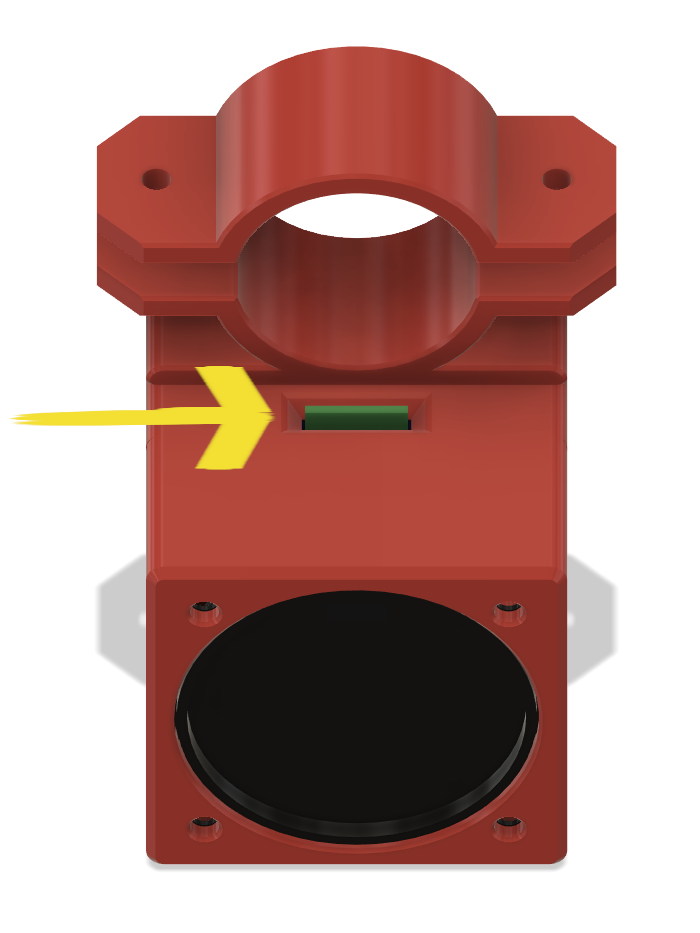
\includegraphics[width=0.25\textwidth]{graphics/sd_arrow.png}
				\end{wrapfigure}

				Once you have transferred your MP3 file to the MicroSD card, you will need to insert the MicroSD card into the walking aid device. You can insert the MicroSD card into the walking aid device by simply sliding the MicroSD card into the slot until you feel a click. The location of the MicroSD card slot can be seen in the image to the right. Once you have inserted the MicroSD card into the walking aid device, you are ready to power on your devices. Ensure that the MicroSD card is connected to the walking aid device before powering the device on.

				\paragraph{Powering on your devices}\mbox{}

				Our current prototype does not include an internal battery, but different battery solutions will be provided as options in future work. For now, the devices require 5V USB power, either from a battery bank, computer system, or phone charger. Once you have powered on your devices, you are ready to begin using the Walking Aid Usage Prompt System. To confirm that the device is functional, you should see the flash of a green LED for about one second.

				Should you notice any other LED light indicators, then please refer to the User Guide \hyperref[sec:user_guide]{here} or head to section \ref{sec:user_guide} for further troubleshooting instructions.

				\subsubsection{To use the vibration reminder system}

				As you are relying on the vibration reminder system, there is no need to utilise a MicroSD card, therefore you can skip to powering on the device. The design of our current prototype means that we will have setup the devices prior to you receiving them to ensure that they are functional for vibration reminders. Future work will be carried out to ensure that a button or switch system is implemented to allow the user to switch between vibration and audio reminders themselves.

				\paragraph{Powering on your devices}\mbox{}

				Our current prototype does not include an internal battery, but different battery solutions will be provided as options in future work. For now, the devices require 5V USB power, either from a battery bank, computer system, or phone charger. Once you have powered on your devices, you are ready to begin using the Walking Aid Usage Prompt System. To confirm that the device is functional, you should see the flash of a green LED for about one second.

				Should you notice any other LED light indicators, then please refer to the User Guide \hyperref[sec:user_guide]{here} or head to section \ref{sec:user_guide} for further troubleshooting instructions.

	\newpage
	\section{User Guide}
	\label{sec:user_guide}

		\subsection{Introduction}

			The Walking Aid Usage Prompt System is a pair of hardware devices that communicate with each other to ensure that dementia patients are utilising their walking aids when walking. The system was designed such that one device is attached to the walking aid device, which includes the MicroSD card reader and external speaker necessary for the reading and playing of the audio reminder. The other device is designed to be worn on the patient's wrist or ankle and is capable of detecting when the patient is walking as well being capable of playing a vibration reminder to the patient if desired. When the wearable device has detected that the patient has walked 5 steps within a 10 second period, the walking aid device will play an audio or vibration reminder to the patient if it is not also moving. 

			This user guide details the necessary steps to setup the devices ready for use along with instructions for troubleshooting if any issues are encountered.

		\subsection{Hardware Requirements}
		\label{subsec:hardware_reqs}

			\paragraph{To use the audio reminder system:}\mbox{}

			\begin{itemize}
				\item MicroSD Card >= 2MB Capacity.
				\item Windows/MacOS/Linux Computer System.
				\item A means to read/write to the SD card from the computer system. For example, a USB to MicroSD card reader.
				\item A microphone to record audio, or a pre-recorded audio file (.MP3)
			\end{itemize}

			\paragraph{To use the vibration reminder system:}\mbox{}

			No additional hardware necessary, please advance to section \ref{subsec:setup_guide}.

		\subsection{Software Requirements}
		\label{subsec:software_reqs}

			\paragraph{To use the audio reminder system:}\mbox{}

			\begin{itemize}
				\item Voice recording software such as Windows Voice Recorder or Audacity. (An alternative could be to record your voice message on a mobile device and transfer it to the computer system).
				\item File explorer software to copy the file to the SD card.
				\item MP3 audio file should be <= 2MB in size.
			\end{itemize}

			\paragraph{To use the vibration reminder system:}\mbox{}

			No additional software necessary, please advance to section \ref{subsec:setup_guide}.

		\subsection{Setup Guide}
		\label{subsec:setup_guide}

			The following section is a full setup guide that can be followed to ensure that the Walking Aid Usage Prompt System is functioning correctly. The setup guide includes similar information and instructions to the quick start guide, however it shall contain more detail. The setup of the devices for use of the vibration reminder system only requires the powering on of the devices, which will be detailed in the latter stages of this user guide. The setup of the devices utilising the audio reminder system requires the completion of the following steps:

			\begin{itemize}
				\item Preparing the MicroSD card for use.
				\item Formatting your MicroSD card
				\item Recording a voice message if one is not prepared already.
				\item Transferring the audio file to the MicroSD card.
				\item Inserting the MicroSD card into the walking aid device.
				\item Powering on the devices.
			\end{itemize}

			If you are intending on utilising the vibration reminder system, then you can click \hyperref[para:powering]{here} or head to the 'Powering on your devices' section. Otherwise, please follow the steps outlined below to ensure that the Walking Aid Usage Prompt System is functioning correctly for audio reminding.

			\subsubsection{Preparing the MicroSD card for use}

				Please ensure before proceeding that the MicroSD card has a capacity of at least 2MB. You can confirm this with the packaging of the MicroSD card or by connecting it to your computer system and checking in the Windows/MacOS/Linux file explorer.

				Before getting started with the transferring of your MP3 file to the SD card, you will need to ensure that you have a means to read/write to the SD card. For example, a USB to MicroSD card reader that can connect to your computer system or mobile device, or computer system with a built in MicroSD card reader.

				\paragraph{Formatting your MicroSD card}\mbox{}

				It is imperative that your MicroSD card is utilising a FAT16/FAT32 file system to ensure that the walking aid device functions correctly. Should your MicroSD card be using a different file system, please format your MicroSD card so that it is using a FAT16/FAT32 file system. WARNING! Formatting your MicroSD card will cause you to lose all of your data currently saved on it. Instructions for formatting your MicroSD card can be found below:

				\begin{itemize}
					\item \href{https://www.bu.edu/comtech/students/technical-guides/hardware/how-to-format-hard-drives/}{Format Instructions}
				\end{itemize}

				Once the MicroSD card has been setup with the FAT16/FAT32 file system, you can proceed to the next step, transferring the audio recording to the MicroSD card.

				\paragraph{Recording a voice message if one is not prepared already}\mbox{}

				Should you already have an audio recording prepared, then please ensure that the audio file is in an MP3 format. We also recommend that the audio file has a 44.1kHz sample rate and a 128kbps bit rate.

				Using voice recording software and a microphone, record your voice message. Recommended voice recording software includes, but is not limited to, the following:

				\begin{itemize}
					\item Windows Voice Recorder
					\item Audacity
					\item Mobile Device Voice Recording App such as Voice Recorder \& Audio Editor by TapMedia Ltd (iOS)
				\end{itemize}

				We recommend that the audio file has a 44.1kHz sample rate and a 128kbps bit rate. This can be set when configuring the voice recording software, or by using software to edit the audio file after it has been recorded.

				We also recommend recording a reminder message to the patient with a friendly voice. Friendly voices are known to provide a higher success rate than generic voices that could further confuse or frighten the patient.

				\paragraph{Transferring your MP3 file to the MicroSD card}\mbox{}

				To transfer from your computer system to the MicroSD card, you will need to ensure that your file explorer software such as Windows Explorer or MacOS Finder ready to use.

				If you have recorded your voice message using a mobile device, you can either transfer your MP3 file to the computer system using a message system such as email or by connecting your mobile device to your computer system via USB. Another option is to connect your MicroSD card to your mobile device using one of the previously mentioned adapters to allow for file transfer.

				Once you have access to writing to your MicroSD card, you are ready to transfer your MP3 file. Please follow the following steps to ensure that your MP3 file is transferred to the MicroSD card correctly to be fully functional with the Walking Aid Usage Prompt System:

				\begin{itemize}
					\item Open the file explorer software and locate your voice recorded MP3 file.
					\item Rename the file to 'reminder.mp3'.
					\item Through the file explorer software, locate your MicroSD card's storage location.
					\item Create a folder on the MicroSD card named 'reminder'.
					\item Copy and paste the 'reminder.mp3' file from your computer system/mobile device to the 'reminder' folder on the MicroSD card.
				\end{itemize}

				\paragraph{Inserting you MicroSD card into the walking aid device}\mbox{}

				\begin{wrapfigure}{R}{0.25\textwidth}
					\vspace{-3.5em}
					\centering
					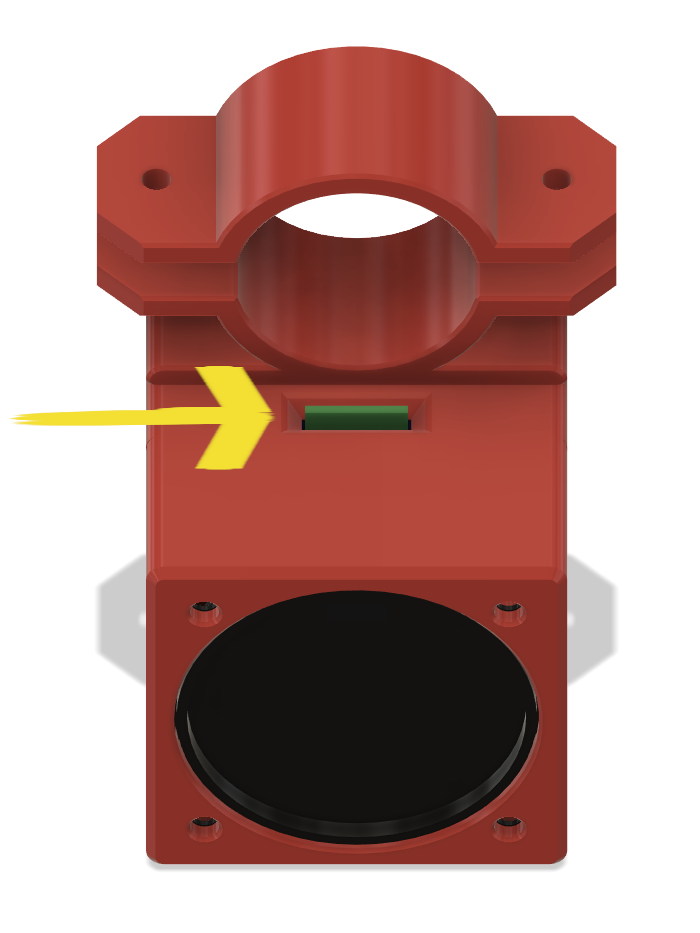
\includegraphics[width=0.25\textwidth]{graphics/sd_arrow.png}
				\end{wrapfigure}

				Once you have transferred your MP3 file to the MicroSD card, you will need to insert the MicroSD card into the walking aid device. You can insert the MicroSD card into the walking aid device by simply sliding the MicroSD card into the slot until you feel a click. The location of the MicroSD card slot can be seen in the image to the right. Once you have inserted the MicroSD card into the walking aid device, you are ready to power on your devices. Please remember that the walking aid device must have a MicroSD card inserted before the device is powered on to ensure that an audio file can be transferred to the device's onboard memory.

				\paragraph{Powering on your devices}\mbox{}
				\label{para:powering}

				If you are intending on using the vibration reminder system then the design of our current prototype means that we will have setup the devices prior to you receiving them to ensure that they are functional for vibration reminders. Future work will be carried out to ensure that a button or switch system is implemented to allow the user to switch between vibration and audio reminders themselves.

				Our current prototype does not include an internal battery, but different battery solutions will be provided as options in future work. For now, the devices require 5V USB power, either from a battery bank, computer system, or phone charger. Once you have powered on your devices, you are ready to begin using the Walking Aid Usage Prompt System. To confirm that the device is functional, you should see the flash of a green LED for about one second.

				Should you notice any other LED light indicators, then please refer to the troubleshooting LEDs guide \hyperref[subsec:troubleshooting_leds]{here} or head to section \ref{subsec:troubleshooting_leds} for further troubleshooting instructions.

		\subsection{Troubleshooting LEDs}
		\label{subsec:troubleshooting_leds}

			\begin{tabular}{ m{0.1\linewidth} m{0.8\linewidth} } 

				\vspace{2em}
				
\includegraphics[width=0.5\linewidth]{graphics/green_circle.png}
				
				& You should see this LED for one second when you initally power on the device. This indicates that your device is functional. \\ 

				\vspace{2em}
				
\includegraphics[width=0.5\linewidth]{graphics/orange_circle.png}
				
				&  You are seeing this LED because the device in question is struggling to connect to the other device. Try powering them down, moving them closer together and restarting them. If you are still experiencing issues, please contact our support team here. \\ 

				\vspace{2em}
				
\includegraphics[width=0.5\linewidth]{graphics/red_circle.png}
				
				& This LED is being displayed as the initialisation of the communication protocol has failed. Please contact our support team here. \\
				 
			\end{tabular}

	\newpage
	\section{Developer Guide}
	\label{sec:developer_guide}

		This section is designed to help developers in the future to build on top of this project, to experiment with further techniques for the main features and to allow them the opportunity to learn from our code and systems to help impact the lives of dementia patients. We understand that this project may be handed onto developers in a professional setting in future, and wanted to offer a section including the necessary details on this project to allow developers to easily understand the code and systems.

		This section will contain details on how we wired both the walking aid and wearable devices, and why we decided to wire the devices the way we did. It will also contain details on the code that we have written and will provide suggestions as to how the code can be improved moving forward. We have developed our code such that classes can be transferred seamlessly for classes that utilise more expensive hardware or more complex libraries to help facilitate the advancement of these systems in future. 

		\subsection{Wiring}
		\label{subsec:wiring}

			We had intended to include a wiring diagram here of the connections between our TinyPICO boards, the accelerometers and the audio shield. However, there seems to be a lack of software that allows for the creation of wiring models for TinyPICO boards. We have therefore decided to include a list of the connections that we have made between the devices. Following this list will be illustrations of the hardware used and their pinouts. Thus, the developer can understand how the hardware is connected and be able to reference the images to understand where the pins are located on them. The following is a list of the necessary wiring between the hardware, with the TinyPICO to ADXL345 Accelerometer section necessary for both the walking aid and wearable devices, and the TinyPICO to I2S Audio Shield necessary only for the walking aid device.

			\subsubsection{TinyPICO to ADXL345 Accelerometer}

				As it was necessary for us to utilise the SPI communication standard for the communication between the TinyPICO board and the I2S Audio Shield in the walking aid device, we were influenced to utilise the I\textsuperscript{2}C communcation standard between the TinyPICO boards and the ADXL345 accelerometer. The full wiring list for the TinyPICO to ADXL345 Accelerometer is shown below.

				\begin{itemize}
					\item TinyPICO 5V Pin (5V) \hspace{2.5em} ---> \hspace{2em} ADXL345 VCC Pin.
					\item TinyPICO Ground Pin (G) \hspace{1.15em} ---> \hspace{2em} ADXL345 GND Pin.
					\item TinyPICO SDA Pin (21)	\hspace{2em} ---> \hspace{2em} ADXL345 SDA Pin.
					\item TinyPICO SCL Pin (22)	\hspace{2.1em} ---> \hspace{2em} ADXL345 SCL Pin.
				\end{itemize}

				We opted not to utilise the INT1 and INT2 interrupt pins for this project, but they do provide an interesting experimental feature for further development work. These pins could be used to trigger a software interrupt on the TinyPICO board, which would allow code to be run in real time when an event has been triggered through the accelerometer.

			\subsubsection{TinyPICO to I2S Audio Shield}

				The TinyPICO to Audio Shield communication utilises the I\textsuperscript{2}S audio communication standard and that was why we opted for this specific wiring communication. It was also a necessity for us to use the SPI communication protocol between the two hardware devices to provide a communication route for the transferring of audio files between the two boards. The full wiring list for the TinyPICO to I2S Audio Shield is shown below.

				\begin{itemize}
					\item TinyPICO 3.3V Pin (3V3) \hspace{2.1em} ---> \hspace{2em} I2S Audio Shield 3.3V Pin (3V3).
					\item TinyPICO Ground Pin (G) \hspace{2em} ---> \hspace{2em} I2S Audio Shield Ground Pin (G).
					\item TinyPICO SS Pin (5) \hspace{4.15em} ---> \hspace{2em} I2S Audio Shield SD SEL Pin (5).
					\item TinyPICO SCK Pin (18) \hspace{2.8em} ---> \hspace{2em} I2S Audio Shield SPI CLK Pin (18).
					\item TinyPICO MI Pin (19) \hspace{3.55em} ---> \hspace{2em} I2S Audio Shield SPI MI Pin (19).
					\item TinyPICO MO Pin (23) \hspace{3.15em} ---> \hspace{2em} I2S Audio Shield SPI MO Pin (23).
					\item TinyPICO DAC 1 Pin (25) \hspace{2em} ---> \hspace{2em} I2S Audio Shield D IN Pin (25).
					\item TinyPICO DAC 2 Pin (26) \hspace{2em} ---> \hspace{2em} I2S Audio Shield LRCLK Pin (26).
					\item TinyPICO TCH 7 Pin (27) \hspace{2em} ---> \hspace{2em} I2S Audio Shield BCLK Pin (27).
				\end{itemize}

		\newpage
		\subsection{Hardware Pinouts}
		\label{subsec:hardware_pinouts}

			The following sections will contain the pinout images for the TinyPICO board, the ADXL345 accelerometer and the I2S Audio Shield. These images are provided for reference with the wiring section in section \ref{subsec:wiring}, to aid in the process of understanding the wiring of our systems and to allow developers to reconfigure the wiring of the devices themselves.

			\subsubsection{TinyPICO Board}

				The following is an image of the pinouts of the TinyPICO board \cite{tinypico}.

				% [H] means put the figure HERE, directly when you input this code.
\begin{figure}[H]
	\centering
	\captionsetup{width=1.0\linewidth}

% We set the width of the figure based on the width of one line of text on the page.
% The value can be tuned to any value in [0.0, 1.0] to scale the image while maintaining its aspect ratio.

	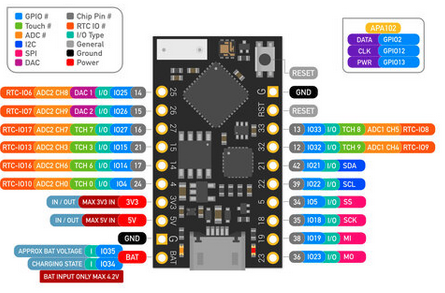
\includegraphics[width=1.0\linewidth]{graphics/tinypico_pinouts.png}

% Caption is defined with a short and long version. The short version is shown in the
% List of Figures section, and the long version is used directly with the figure.
	\caption[TinyPICO Pinouts]{An illustration of the TinyPICO pinouts provided by \cite{tinypico}}

% For figures label should be defined after the caption to ensure proper figure numbering.
	\label{fig:tinypico_pinouts}

\end{figure}

			\newpage
			\subsubsection{ADXL345 Accelerometer}

				The following is an image of the pinouts of the ADXL345 accelerometer \cite{components101}.

				% [H] means put the figure HERE, directly when you input this code.
\begin{figure}[H]
	\centering
	\captionsetup{width=1.0\linewidth}

% We set the width of the figure based on the width of one line of text on the page.
% The value can be tuned to any value in [0.0, 1.0] to scale the image while maintaining its aspect ratio.

	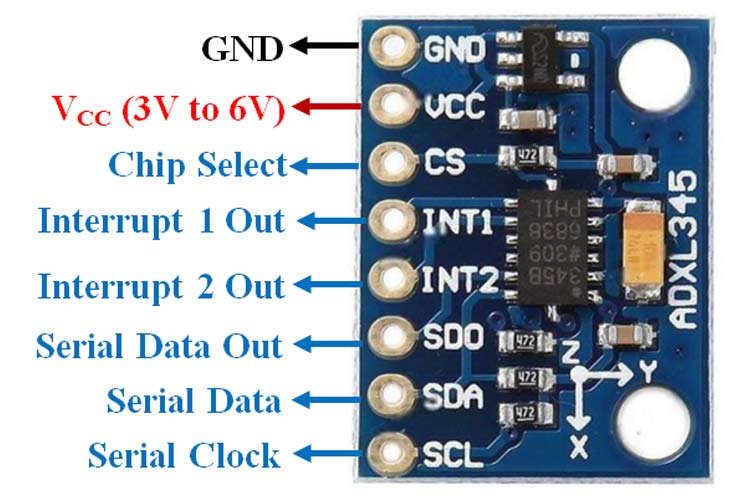
\includegraphics[width=0.75\linewidth]{graphics/accel_pinouts.jpg}

% Caption is defined with a short and long version. The short version is shown in the
% List of Figures section, and the long version is used directly with the figure.
	\caption[ADXL345 Accelerometer Pinouts]{An illustration of the ADXL345 accelerometer pinouts provided by \cite{components101}}

% For figures label should be defined after the caption to ensure proper figure numbering.
	\label{fig:accel_pinouts}

\end{figure}

			\newpage
			\subsubsection{I2S Audio Shield}

				The following is an image of the pinouts of the I2S audio shield \cite{unexpected_maker}.

				% [H] means put the figure HERE, directly when you input this code.
\begin{figure}[H]
	\centering
	\captionsetup{width=1.0\linewidth}

% We set the width of the figure based on the width of one line of text on the page.
% The value can be tuned to any value in [0.0, 1.0] to scale the image while maintaining its aspect ratio.

	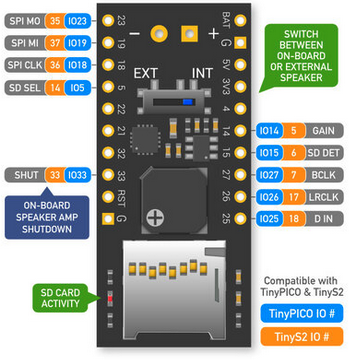
\includegraphics[width=0.75\linewidth]{graphics/audioshield_pinouts.png}

% Caption is defined with a short and long version. The short version is shown in the
% List of Figures section, and the long version is used directly with the figure.
	\caption[I2S Audio Shield Pinouts]{An illustration of the I2S audio shield pinouts provided by \cite{unexpected_maker}}

% For figures label should be defined after the caption to ensure proper figure numbering.
	\label{fig:audioshield_pinouts}

\end{figure}

		\newpage
		\subsection{Software Development}

			This section is designed to help the developer understand what each class within the software system does and how they can be altered to incorporate different technologies that could potentially improve the system in future. Each breakdown of the classes will include an overview of what the class does, and what particular changes can be made to adjust the system.

			\subsubsection{WalkAidAccelerometer/WearableAccelerometer}

				These classes are used to operate the walking and movement detection features of the wearable and walking aid devices. They currently utilise a system that detects changes in gravity over a specified threshold as steps. Those steps are recorded as the steps those devices have taken and signify whether they are moving or not. Issues relating to this system can also be identified in high end mobile step counters, where the quick movement of the mobile device without actually walking can cause steps to be detected.

				Listing \ref{lst:accel} demonstrates how the code is implemented to detect changes in gravity and call the code that increments the step counter on the wearable device and the last step time updater on the walking aid device. This code can be easily replaced with code that detects changes in acceleration for example. An interesting alternative here could be to implement distance tracking between the two devices with the accurate Ultra wideband technology currently on offer. However, this technology would add to your budget. 

				\lstinputlisting[language=C++, caption=Code to detect steps through the ADXL345's built-in single tap detection feature., label=lst:accel]{listings/tap_detection.cpp}

				Both accelerometer classes also contain initialisations of the accelerometer, which is used to set the threshold for the single tap detection feature. We encourage the developers to experiment with different thresholds to see how the system performs for your specific needs. A further feature that could be experimented with is the use of the interrupt signals sent by the accelerometer. Utilising the INT1 or INT2 pins on the ADXL345 could allow the user to call a function in real time when an event has been triggered through the accelerometer.

				Further documentation for these classes can be viewed in sections \ref{subsec:WalkAidAccelerometer} and \ref{subsec:WearableAccelerometer}.

			\subsection{WalkAidCommunications/WearableCommunications}

				These classes are used to define the communication behaviours between the walking aid and wearable devices. As mentioned previously, we opted to utilise ESP-Now as our communication protocol, but this technology can be easily transferred to the developer's preferred technology such as Bluetooth. The classes in their current form include an init class that initialises the necessary details for ESP-Now to function correctly within this system. This includes the assigning of peer devices and messages that should be sent to those peer devices. 

				Within the main sketch files of each device, we include the callback function OnDataRecv, which is called when ESP-Now detects a message. It is here that the developer can adjust the behaviour of the system when the message received. For example, we currently use the code in listing \ref{lst:callback} on the walking aid device to set a boolean to true, which in turn allows the next run of the Arduino loop function to check if the walking aid is moving. This can be adjusted however to incorporate the needs of the developer. For example, the developer could instead opt to use a different method for movement detection and have that function called within the callback function.

				\lstinputlisting[language=C++, caption=A callback function called when the walking aid device detects a message., label=lst:callback]{listings/callback.cpp}

				Further documentation for these classes can be viewed in sections \ref{subsec:WalkAidCommunications} and \ref{subsec:WearableCommunications}.

			\subsection{WalkAidAudio}

				The WalkAidAudio class handles the initialisation of the SDToSPIFFS class, calls for the audio file to be transferred from the SD card to the SPIFFS file system, and then calls for the audio file to be played when necessary. The class currently utilises a select number of generator classes to allow the ESP32 to interpret the MP3 file. The developer can adjust these classes to allow for further audio file formats to be interpreted also.

				The playing of the audio file requires the reinstantiation of these audio generators and decoders before allowing the audio to be played correctly.

				Further documentation for this class can be viewed in section \ref{subsec:WalkAidAudio}.

			\subsection{SDToSPIFFS}

				To allow for the transferral of the MP3 file from the MicroSD card to the SPIFFS file system, the SDToSPIFFS class is used. The class utilises the SdFat library discussed in section \ref{subsec:sdfat}. We opted to utilise this class due to the inefficiency of Arduino's SD library, we highly recommend that the developer avoids the use of the Arduino SD library due to these inefficiency reasons. Our current system requires that the MicroSD card is within the MicroSD card slot of the walking aid device whenever it is powered on. This is due to the fact that the SPIFFS file system is volatile and therefore data within it is deleted when the device powers down. A future advancement to this could involve the developer adjusting our code in listing \ref{lst:transfer} to allow for the transferral of the MP3 file to a persistent storage location, or to include code that detects when a MicroSD card has been inserted and have the transferral process take place at that point. 

				\lstinputlisting[language=C++, caption=Code to transfer the MP3 file from the MicroSD card to the SPIFFS file system., label=lst:transfer]{listings/transfer.cpp}

				Further documentation for this class can be viewed in section \ref{subsec:sdtospiffs}.

			\subsection{Sketch Files}

				The sketch file for each device contains the functions necessary to allow the devices to be developed through Arduino. The setup function of each class instantiates the required libraries for the full desired functionality of the systems. The loop function for the wearable device repeatedly calls the check for step function where steps are detected and added to the counter, and calls for messages to be sent to the walking aid device are made should a reminder need to be played.

				The loop function for the walking aid device is a little more complex as it incorporates the functionality for checking if the walking aid had been moved in the last 10 seconds and if not, waits to see if the walking aid is moved in the next 10 seconds before deciding to play a reminder or not. The code for the walking aid loop function can be viewed in listing \ref{lst:loop}. The main area we feel that the developer could experiment with here is to implement the accelerometer interrupt feature to allow movements to be responded to in real time rather than having to wait for the loop function to be called each time to have movements detected.

				\lstinputlisting[language=C++, caption=The loop function of the walking aid sketch file., label=lst:loop]{listings/loop.cpp}

				Further documentation for these sketch files can be viewed in sections \ref{subsec:sketch_walking_aid} and \ref{subsec:sketch_wearable}.
